\chapter{Zweite Methode} \label{cha:ZweiteMethode}

In diesem Kapitel wird die Realisierung des zweiten Verfahrens eingegangen. Zuerst wird die allgemeine Struktur dieser Methode beschrieben. Dies liefert ein grobes Verständnis der Struktur und des Arbeitsprinzips der gesamten Methode. Anschießend läuft eine Erklärung der Bildverarbeitungen im Detail. Diese besteht aus folgenden Teilen: Binarisierung, Morphologie Operation und Canny Kannten Detektion. In diesem Abschnitt wird erläutert, wie diese Operationen funktionieren und was der Sinn dieser Behandelungen ist. Schließlich wird eine Linienextrahierungsmethode$ (Hough und Radon Transformation) $ detailliert vorstellen. 

\section{Allgemeine Struktur} 

Anders als bei der vorherigen Methode, indem durch die  Charakteristiken des QR Musters die Modulationsbereiche detektiert wurden, wird hier eine neue Strategie mit Hilfe geometrischen Eigenschaften des Modulationsbereichs verwendet. Es ist bekannt, dass im DaVid System durch Aufnahme des Inhalts auf dem Bildschirm die versteckten Daten erkannt werden können. Dann entspricht der Modulationsbereich tatsächlich dem Bildschirmbereich, der im Allgemeinen über die Form von einem Rechteck verfügt. Deswegen kann hier das Problem eines Detektierens des Modulationsbereichs in ein Problem des Detektierens eines Rechtecks umgewandelt werden. Außerdem, wegen der geometrischen Eingenschaften des Rechtecks, welches aus 2 paaren paralleler Linien besteht, lassen das Problem zu ein Linienextrahierungsproblem. Das heißt, diese Methode basiert auf dem extrahieren der Linien auf dem Bild, um den endgültigen Modulationsbereich zu erkennen und zu bestimmen. Abbildung \ref{fig:Strukturdiagramm} zeigt das Strukturdiagramm dieses Verfahrens.

\begin{figure}[H]
 \centering 
 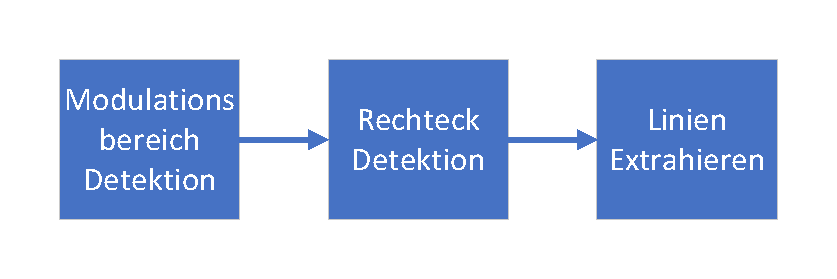
\includegraphics[keepaspectratio,width=1.0\textwidth]{images/4_ZweiteErfahrung/Strukturdiagramm.pdf}
 \caption{Strukturdiagramm}
 \label{fig:Strukturdiagramm für zweite Methode}
\end{figure}


Das Objekt, welches mit dieser Methode bearbeitet wird, ist eine Reihe von Bildern, die von einer Handkamera mit Stativ aufgenommen wurde. Durch des Stativ können diese Bilder in dasselbe Koordinatensystem sein. Mit gegenseitiger Subtraktion wird eine Reihe Differenzbilder erhalten. Durch das Wissen des vorherigen Kapitels, wird die $``Energie"$ hauptsächlich aus dem Modulationsbereich gewonnen. Durch Addition der Differenzbild mit der meisten $``Energie"$ kann ein zu detektierendes Bild erhalten werden um die folgende Operation durchzuführen. Diese Teilbereiche sind schon im vorherigen Kapitel beschrieben und werden hier nicht ins Detail erklärt. Um den Modulationsbereich vom Bild hervorzuheben, wird das zu detektierendes Bild binarisiert, dadurch wird das Bild in zwei Teile geteilt, ein für das Objekt (hier der Modulationsbereich) und ein für den Hintergrund (hier der Bereich um den Modulationsbereich). Danach wird zur Beseitigung der zahlreichen Unvollkommenheiten (hier die kleinen Punkte und Lücken), die von Rauschen und Fehlern verursacht werden, wird hier eine morphologische Behandelung benötigt, welche auf der Form und Struktur des Objekts basiert. Als Nächstes soll der Modulationsbereich erkannt werden. Um diese zu implementieren, muss die rechteckige Grenze zwischen dem Modulationsbereich und dem Hintergrundbereich gefunden werden. Mit Hilfe einer Kantenextraktionsmethode, also dem Canny-Algorithmus, werden im Bild nur die Kanten übernommen, die der Grenze des Modulationsbereichs entsprechen. Die Grenze des Modulationsbereichs hat eine rechteckige Form, bestehend aus vier Linien. Das Hough- und Radon-Transformationsverfahren wird verwendet, um alle zwei geraden Linien in der horizontalen Richtung bzw. der vertikalen Richtung zu erfassen. Schließlich wird das endgültige Rechteck, also der Modulationsbereich, durch die vier geraden Linien bestimmt. Das Flussdiagramm wird in Abbildung \ref{fig:Flussdiagramm der zweite Methode} gezeigt. Die Details jedes Teils werden in den folgenden Abschnitten beschrieben.

\begin{figure}[H]
 \centering 
 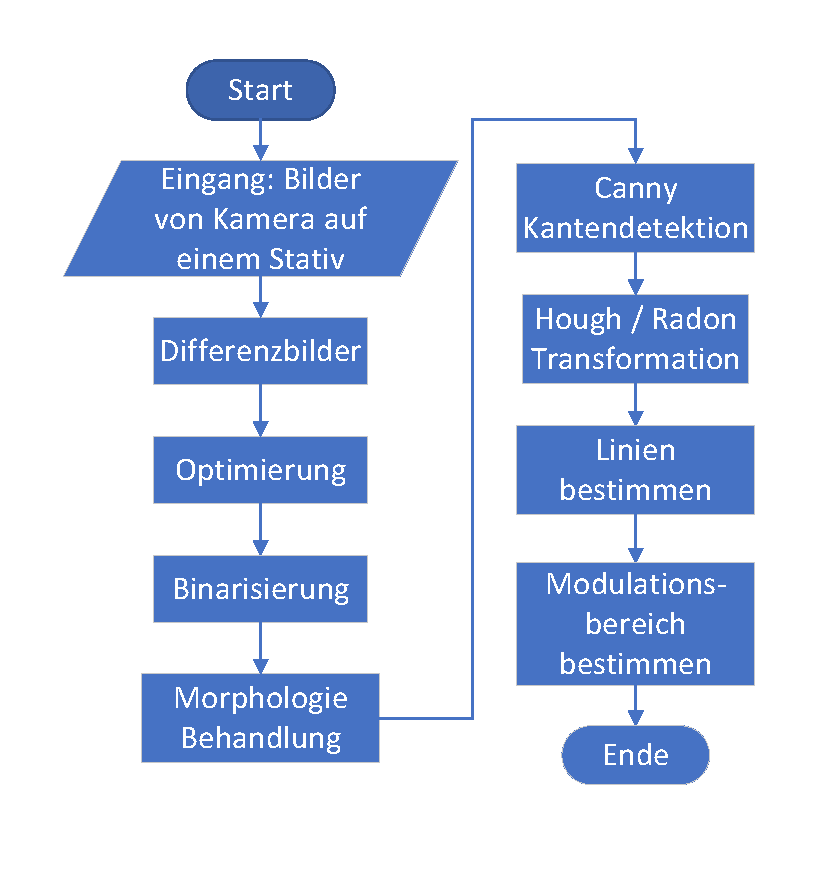
\includegraphics[keepaspectratio,width=1.0\textwidth]{images/4_ZweiteErfahrung/Flussdiagrammsum.pdf}
 \caption{Flussdiagramm der zweite Methode}
 \label{fig:Flussdiagramm der zweite Methode}
\end{figure}

\section{Binarisierung}

In diesem Abschnitt wird der Binarisierungsvorgang der Bildverarbeitung beschrieben. Um den Modulationsbereich zu detektieren, muss dieser zuerst vom Bild hervorgehoben werden. Anschießend kann mit einer Binarisierungs Operation dieser Vorgang implementiert werden, indem das Bild in zwei Teile geteilt wird, ein Teil mit dem Pixelwert 1 für den Modulationsbereich und der andere Teil mit dem Pixelwert 0 für den umgebenden Hintergrund. Schließlich kann der Modulationsbereich mit einigen weiteren Operationen wie morphologische Behandelung, Kanten Detektion behandelt werden.

In der digitalen Bildverarbeitung nehmen binäre Bilder eine ausschlaggebende Position ein. Viele Anwendungen der digitalen Bildverarbeitung können als binäre Probleme betrachtet werden. Um binäre Bilder zu verarbeiten und zu analysieren, wird zunächst das Graustufenbild digitalisieren, um ein binäres Bild zu erhalten. Wenn das Bild weiterverarbeitet wird, bezieht sich die Sammeleigenschaft des Bildes nur auf die Position des Pixels, dessen Pixelwert 0 oder 1 ist, sodass der mehrstufige Wert des Pixels ist nicht länger vertreten ist um die Verarbeitung zu vereinfachen. Darüber hinaus ist die Menge an Datenverarbeitung und Komprimierung gering. 

Um ein ideales Binärbild zu erhalten, werden im Allgemeinen geschlossene, zusammenhängende Grenzen verwendet, um Bereiche zu definieren die sich nicht überlappen. Hier ein einfaches Beispiel zur Veranschaulichung des Binarisierungsvorgang gegeben. In einem bimodalan Histogramm eines Bildes, wie in Abbildung \ref{fig:Histogramm eines einfachen Beispiels}, gibt es zwei scharfe Wellenberg, einen für das Objekt und einen für den Hintergrund. Die Binarisierungsschwelle T wird genau an die tiefste Stelle zwischen den beiden Wellenbergen gelegt. 

\begin{figure}[htb]
 \centering 
  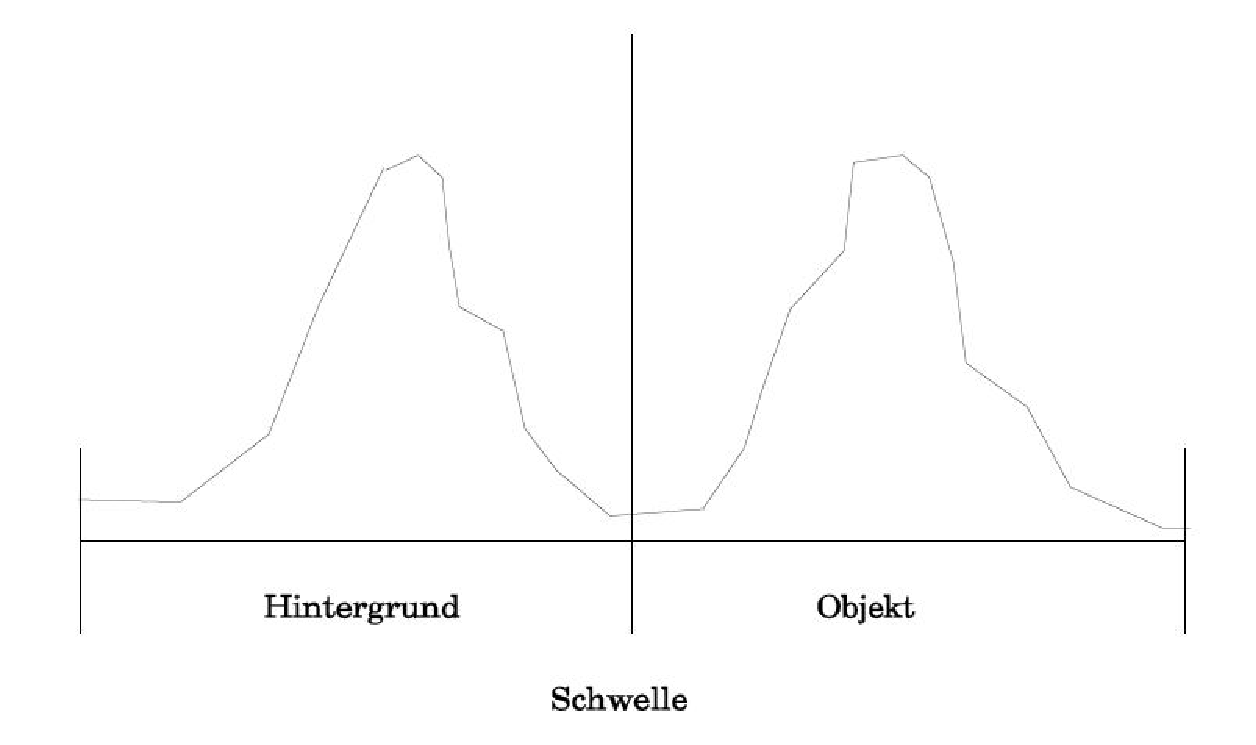
\includegraphics[keepaspectratio,width=0.6\textwidth]{images/4_ZweiteErfahrung/Binar/binar.pdf}
 \caption{Histogramm eines einfachen Beispiels}
 \label{fig:Histogramm eines einfachen Beispiels}
\end{figure} 

Alle Pixel, deren Graustufe größer oder gleich dem Schwellenwert T ist, werden zu einem bestimmten Objekt zugeordnet und deren Pixelwert auf 1 gesetzt. Andernfalls werden diese Pixel aus dem Objektbereich ausgeschlossen und deren Pixelwert auf 0 gesetzt, was den Hintergrund bzw. den Ausnahmeobjektbereich anzeigt. Die Formel dazu lautet:

\begin{equation}
  y(x) =
  \begin{cases} 
  0,   & \mbox{für }x < T \\
  1, & \mbox{sonst}
  \end{cases}
\end{equation}

In der Praxis ist das Histogramm aufgrund der Helligkeit und Inhalt des Bildes nicht der obige bimodale Fall. Dies erfordert auch, dass die geeignete Binarisierungsmethode entsprechend den tatsächlichen Bedürfnissen im Binarisierungsprozess auswählt wird. Als folgende werden einige in dieser Arbeit versuchte Binarisierungsmethoden vorgestellt.

\textbf{Grundlegende globale Schwelle Methode}

Die grundlegende globale Schwellenmethode ist eine Erweiterung der festen Schwellenmethode, die vorher beschrieben wurde. Wenn die Histogrammspitzen und -täler des Bildes offensichtlich sind und Doppelpeaks aufweisen, ist diese Methode effektiver. Basiert auf der visuellen Überprüfung des Histogramms und der Erhaltung des Schwellenwerts durch eine iterative Methode. Die grundlegende Algorithmus ist wie folgt:

1. Wahl eines Parameters t und einen anfänglichen Schwellenwert $ T_{0} $, wobei der Durchschnitt der maximalen Grauwerte $ l_{max} $ und minimalen Grauwerte  $ l_{min} $ verwendet wird. 
\begin{equation}
 T_{0} = (l_{max}+l_{max})/2 
\end{equation}
2. Segmentieren des Bildes mit dem Schwellenwert $ T_{0} $. Dadurch besteht das Bild aus zwei Teilen: $ G_{1} $ besteht aus den Pixeln mit dem Grauwert größer als $ T_{0} $ und $ G_{2} $ aus deren, mit dem Grauwert kleiner oder gleich $ T_{0} $.

3. Berechnen des durchschnittlichen Grauwerts aller Pixel in $ u_{1} $ und $ u_{2} $ und den neuen Schwellenwert $ T_{1} $.
\begin{equation}
 T_{1} = (u_{1}+u_{2})/2
\end{equation}
4. Falls $ |T_{0} - T_{1}| < t $, dann ist $ T_{1} $ der optimale Schwellenwert. Andernfalls wird $ T_{1} $ zu $ T_{0} $ zugewiesen und die Schritte $ 2-4 $ werden wiederholt, bis der optimale Schwellenwert gefunden ist.

Abbildung \ref{fig:Binarisierung mit globalen Schwellenwertmethode} zeigt ein Binarisierungs Beispiel mit globalen Schwellenwertmethode.

\begin{figure}[H]
 \centering 
  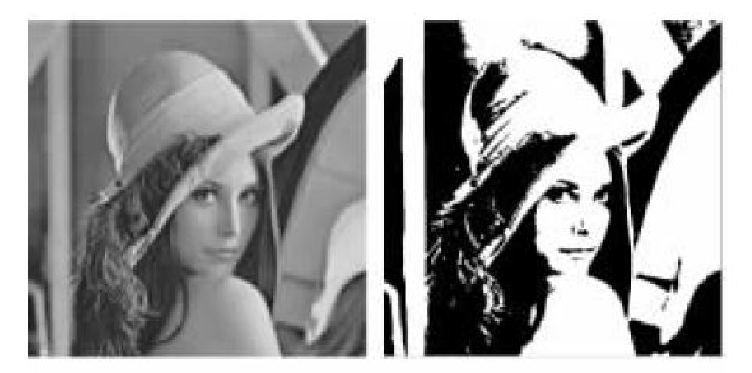
\includegraphics[keepaspectratio,width=0.6\textwidth]{images/4_ZweiteErfahrung/Binar/global.pdf}
 \caption{Binarisierung mit globalen Schwellenwertmethode}
 \label{fig:Binarisierung mit globalen Schwellenwertmethode}
\end{figure} 

\textbf{Grundlegende lokale Schwellenwert Methode}

Ein Bildgebungsfaktor ungleichmäßiger Helligkeit bewirkt, dass ein Histogramm, welches ansonsten für eine effiziente Segmentierung geeignet wäre, ein Histogramm wird, das nicht effektiv mit einem einzigen globalen Schwellenwert segmentiert werden kann.

Das Verfahren zur Verarbeitung besteht darin, das Bild weiter in Unterbilder zu unterteilen, um verschiedene Unterbilder mit unterschiedlichen Schwellenwerten zu segmentieren. Diese Methode wird als grundlegende adaptive Schwellenwert-Binarisierungsmethode bezeichnet. Das Hauptproblem bei diesem Ansatz besteht darin, das Bild zu unterteilen und den Schwellenwert für das resultierende Teilbild abzuschätzen. Da die Schwelle für jedes Pixel von dem Pixel in der Untergruppe abhängt ist die Position im Bild, also solche Schwellen, adaptiv. 

Das Verfahren zum Unterteilen von Unterbildern wird für das Bild übernommen. Hier werden drei Arten von Unterteilungsverfahren ausgewählt, Unterbilder einer Größe von $ 32\times32,4 \times4,16\times16 $ Pixelwerden jeweils geteilt und die durchschnittliche Graustufe der Unterbilder wird als ein Schwellenwert für die Binarisierung ausgewählt. Das Ergebnis wird in Abbildung \ref{fig:Binarisierung mit lokalen Schwellenwertmethode} gezeigt.

\begin{figure}[H]
 \centering 
  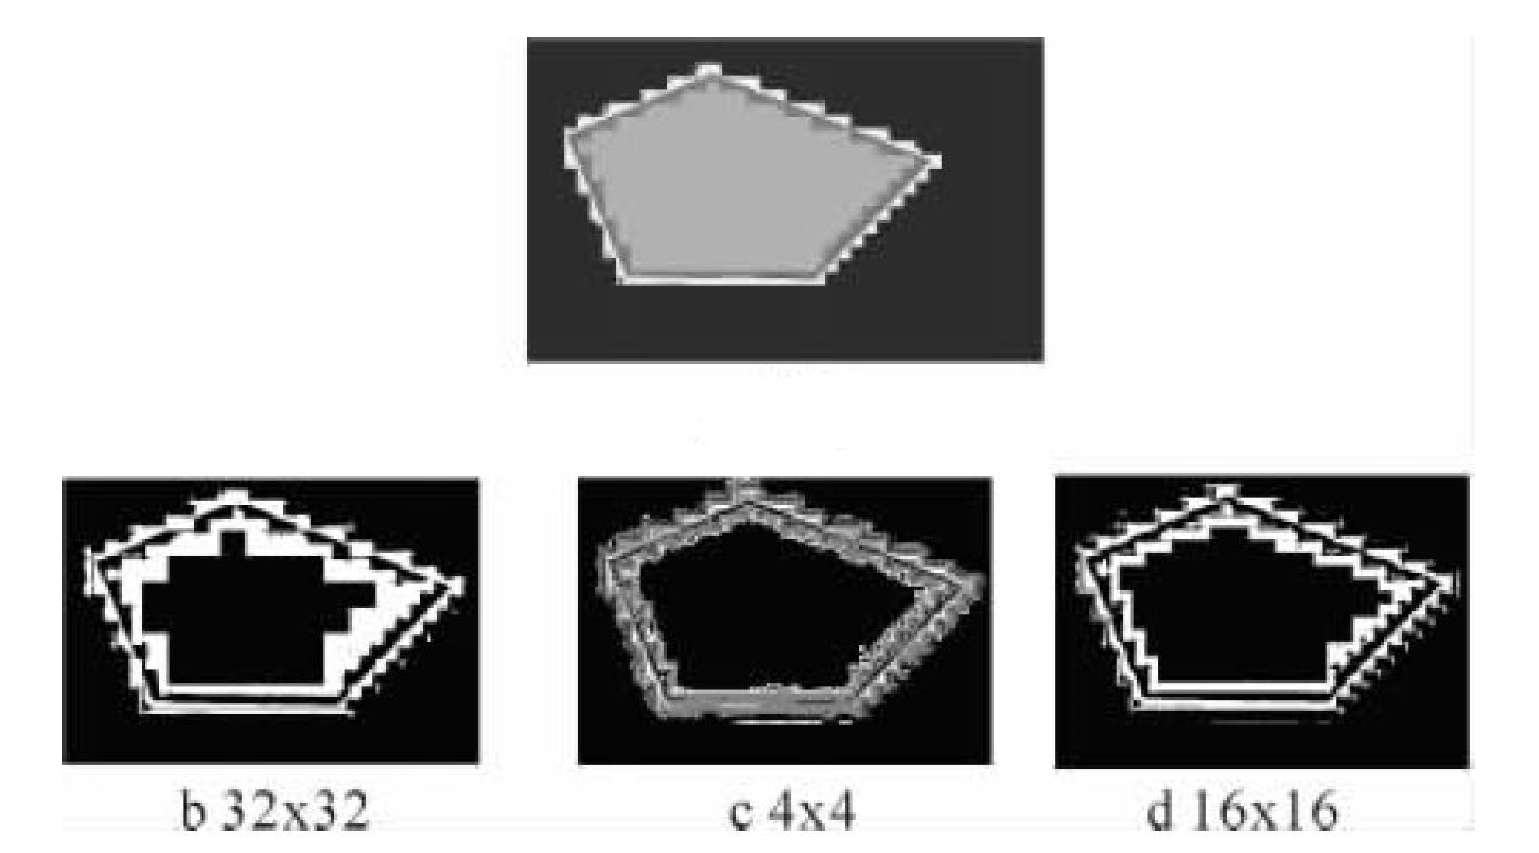
\includegraphics[keepaspectratio,width=0.6\textwidth]{images/4_ZweiteErfahrung/Binar/adaptive.pdf}
 \caption{Binarisierung mit lokalen Schwellenwertmethode}
 \label{fig:Binarisierung mit lokalen Schwellenwertmethode}
\end{figure} 

\textbf{Otsu adaptive Schwellenmethode}

Otsu\cite{Ostu}, auch bekannt als die maximale Interklassenvarianz, wurde 1979 vom japanischen Gelehrten Otsu vorgeschlagen und ist eine adaptive Schwellenwertbestimmungsmethode, die auch als Otsu bekannt ist.

Die Grundidee des Otsu-Algorithmus ist, das Histogramm des Bildes, gemäß der Varianz zwischen dem Vordergrund und dem Hintergrund zu verwenden, um den optimalen Schwellenwert dynamisch zu bestimmen. Die Anzahl der Pixeln in einem Bild ist N und die Graustufe $ L(0,1,...,L-1) $. Die Anzahl der Pixel mit dem Grauwert i ist $ n_{i} $, dadurch ist die Wahrscheinlichkeit von i $ p_{i} = \frac{n_{i}}{N} $. Für das Bild stellt das T Segmentierungsschwellenwert zwischen Vordergrund und Hintergrund dar. Der Vordergrund entspricht den Grauwerten von 0 zu $ T-1 $, dagegen der Hintergrund den Grauwerten von T zu $ L -1 $.

Die Wahrscheinlichkeit des Vordergrundgebiets $ W_{0} $ und des durchschnittlichen Grauwerts $ U_{0} $ sind
\begin{equation}
  w_{0} = \sum_{i=0}^{T-1} p_{i},\quad u_{0} = \sum_{i=0}^{T-1} ip_{i}/w_{0}
\end{equation}

Die Wahrscheinlichkeit der Hintergrundpunkte $ W_{1} $ und des durchschnittlichen Grauwerts $ U_{1} $ sind
\begin{equation}
  w_{1} = \sum_{i=T}^{L-1} p_{i} = 1-w_{0},\quad u_{1} = \sum_{i=T}^{L-1} ip_{i}/w_{1}
\end{equation}

Dann ist der gesamte durchschnittliche Grauwert des Bildes
\begin{equation}
• u = w_{0}u_{0} + w_{1}u_{1}
\end{equation}

Die Infra-Klassen-Varianz ist definiert als
\begin{equation}
•\sigma^2 = w_{0}(u_{0} - u)^2 + w_{1}(u_{1} - u)^2 = w_{0}w_{1}(u_{0} - u_{1})^2
\end{equation}

Wenn der Schwellenwert T sich zwischen 0 und $ L-1 $ befindet und $ \sigma^2 $ das Maximum ist, ist das entsprechende T der optimale Schwellenwert. Beispielsweise wird in Abbildung \ref{fig:Binarisierung mit globalen Schwellenwertmethode} gezeigt.

\begin{figure}[H]
 \centering 
  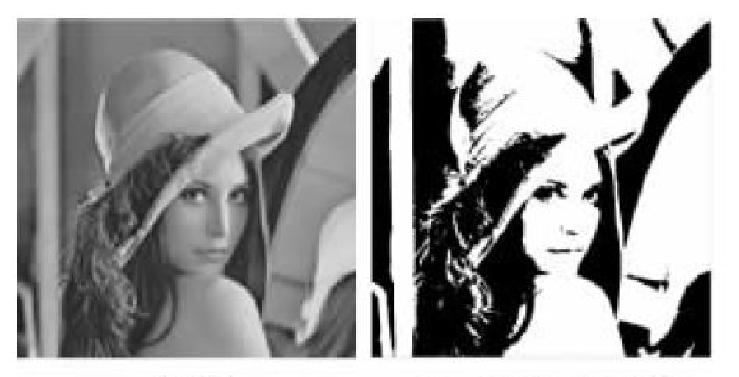
\includegraphics[keepaspectratio,width=0.6\textwidth]{images/4_ZweiteErfahrung/Binar/Ostu.pdf}
 \caption{Binarisierung mit Ostu}
 \label{fig:Binarisierung mit globalen Schwellenwertmethode}
\end{figure} 

Die Ostu-Methode verwendet Grauwerthistogramme zur Bestimmung des Schwellenwerts. Es ist eine automatische nicht-parametrische Schwellenauswahlmethode. Diese Methode ist einfach durchzuführen, wird nicht von der Kontrast- und Helligkeitsänderung unter bestimmten Bedingungen beeinflusst und kann das Objekt zufriedenstellend vom Hintergrundbereich trennen.

Abbildung \ref{fig:binarisierungbild} zeigt Binärbild nach einer Binariesieung Operation mit Ostu.

\begin{figure}[H]
 \centering 
  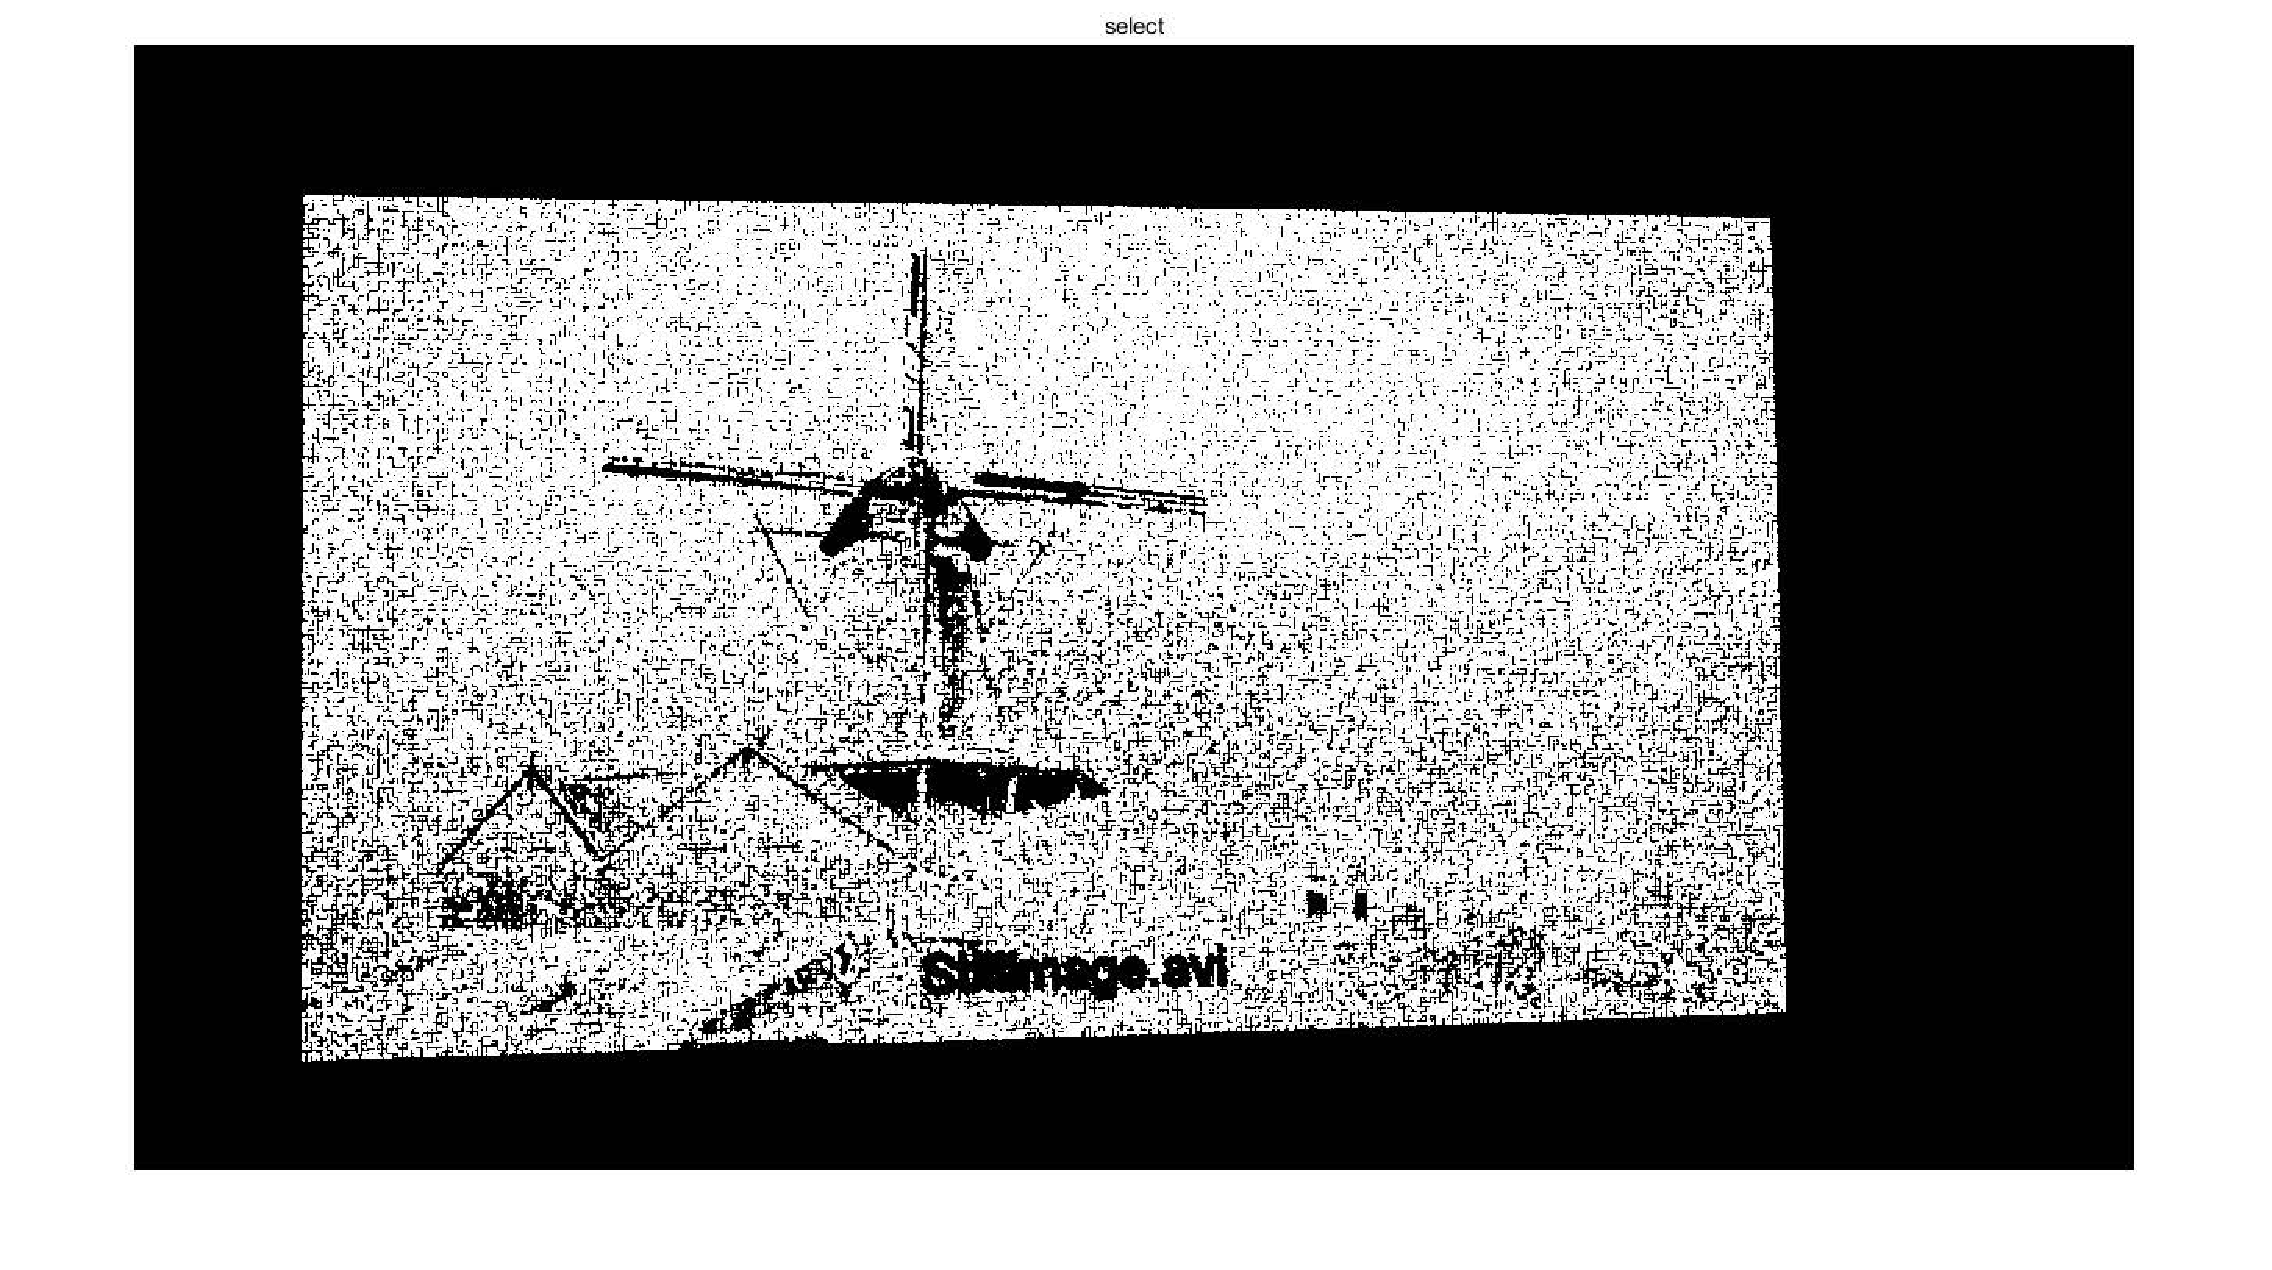
\includegraphics[keepaspectratio,width=1.0\textwidth]{images/4_ZweiteErfahrung/binar/binarisierung.pdf}
 \caption{Binärbild mit Ostu}
 \label{fig:binarisierungbild}
\end{figure} 



\section{Morphologie}

Nach der Binarisierung kann das Bild über zahlreiche Unvollkommenheiten verfügen. Insbesondere ist das Binärbild, welches durch einfache Schwellenwerte generiert wurde, durch Rauschen und Fehlern verzerrt. Die morphologische Bildverarbeitung verfolgt das Ziel, diese Unvollkommenheiten zu beseitigen indem Form und Struktur des Objekts berücksichtigt werden.

Morphologische Operationen arbeiten auf der Grundlage der Mengenoperation und hängen von der relativen Ordnung des Pixelwerts ab. Diese Eigenschaft macht es besonders geeignet für die Verarbeitung von Binärbildern. Natürlich ist die Mengenoperation gültig für alle Graustufenbilder. Hier in dieser Arbeit werden nur binarisierte Bilder benutzt. Es erstellt ein neues Binärbild, bei dem das Pixel nur dann einen nicht-Null Wert hat, wenn die Operation an dieser Position im Eingabebild erfolgreich war.

Die Eingabedaten für die mathematischen morphologischen Operationen sind zwei Bilder: das zu bearbeitende Bild A und ein Strukturelement B. B ist normalerweise eine kleine Pixelmatrix mit jeweils einem Wert von Null oder Eins. Einige Eigenschaften des Strukturelements werden wie folgt gewählt.

\begin{itemize}
\item Die Matrixdimensionen geben die Größe des Strukturelements an.
\item Das Muster, das aus Einsen und Nullen besteht, gibt die Form des Strukturelements an.
\item Ein Ursprung des Strukturelements ist üblicherweise ein Pixel innerhalb des Strukturelements, es verlassen auch außerhalb des Strukturelements liegen. 
\end{itemize}

Eine übliche Anwendung besteht darin, dass der Ursprung ungerader Dimensionen der Pixelmatrixstellen und den Ursprung als das Zentrum der Matrix definiert werden. Einige grundlegende Strukturelemente sind wie folgt:

\begin{figure}[H]
 \centering 
  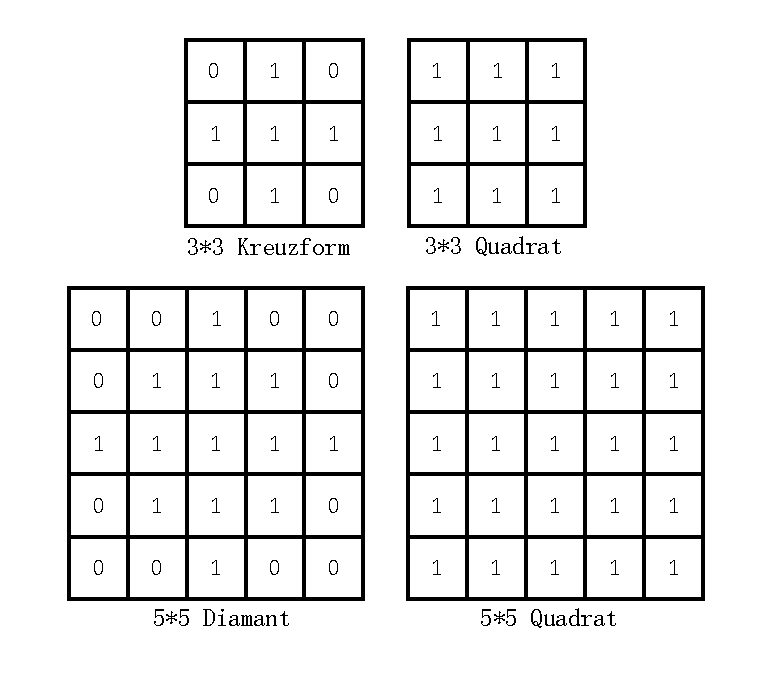
\includegraphics[keepaspectratio,width=0.35\textwidth]{images/4_ZweiteErfahrung/Morphological/strelement.pdf}
 \caption{Einige grundlegende Strukturelemente}
 \label{fig:Strukturelemente}
\end{figure} 

Zuerst werden die zwei grundlegenden morphologischen Operatoren, Erosion und Dilatation, beschrieben. Anschließend werden die darauf basierenden Operationen, die als Öffnung und Schließung bekannt sind, vorgestellt.

\textbf{Dilatation}

Die Dilatation Operation bewirkt, dass das Objekt nach groß wächst. Das Wachstum hängt von der Art und Form des Strukturelements ab. Die Formel einer Dilatation wird dargestellt als:

\begin{equation}
•A \oplus B =\lbrace z \mid \widehat{(B)_z} \cap A \ne \varnothing \rbrace  
\end{equation}

Hier ist $ \widehat{(B)_z} $ das Strukturelement B, welcher seinen Ursprung reflektiert und um z verschoben ist. Die entsprechende Dilatation für das Bild A mit B ist die Menge aller Verschiebungen z, wo $ \widehat{B} $ und A mindestens ein gemeinsames Element haben. Das Ergebnis der Dilatation ist dazu da, um Pixel um die Grenze des Objekts hinzuzufügen. Außerdem wird die Dilatation Operation im wesentlichen verwendet, um die Löcher (fehlende Pixel) in einem soliden Objekt zu füllen. Dieser beeinflusst die Intensität an einem Bereich und kann als ein Unschärfe Effekt bezeichnet werden, nämlich ein räumlicher Tiefpassfilter der beim linearen Filtern des Bildes verwendet wird. Abbildung \ref{fig:Dilatation und Erosion} zeigt eine typische Dilatation Operation.

\begin{figure}[H]
 \centering 
  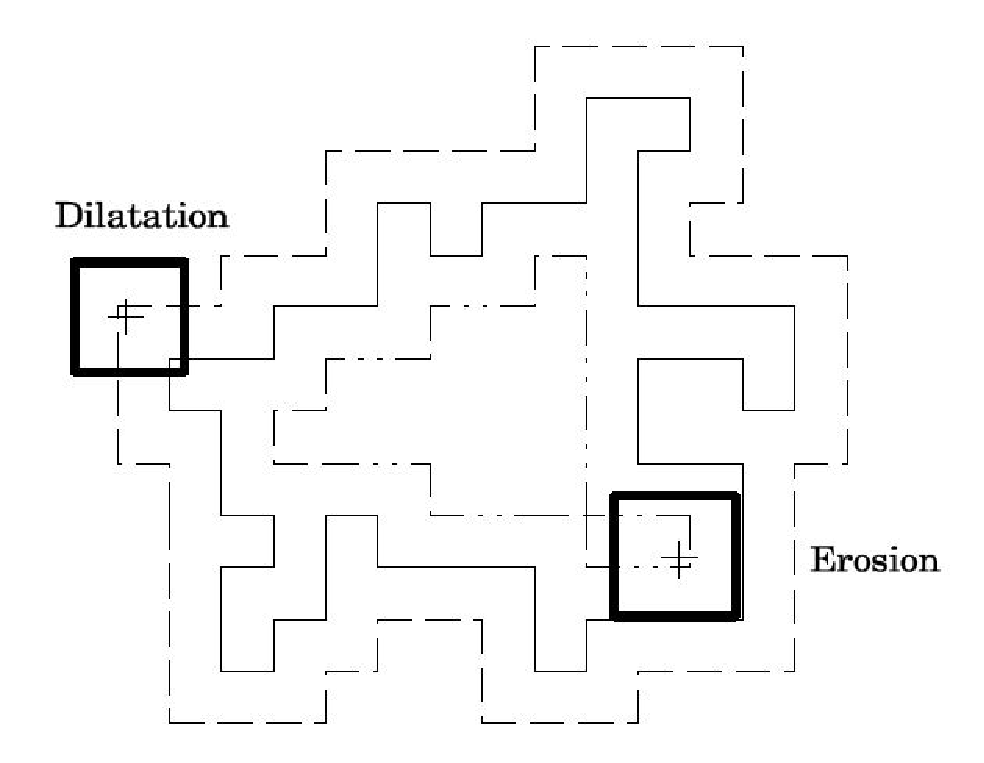
\includegraphics[keepaspectratio,width=0.8\textwidth]{images/4_ZweiteErfahrung/Morphological/DilatationundErosion.pdf}
 \caption{Dilatation und Erosion}
 \label{fig:Dilatation und Erosion}
\end{figure} 


\textbf{Erosion}

Der Operationseffekt einer Erosion ist genau das Gegenteil von dem einer Dilatation. Die Erosion Operation bewirkt, dass das Objekt nach klein werden. Die Erosion eines Bildes A ist durch das Strukturelement B definiert als 
\begin{equation}
•A \ominus B =\lbrace z \mid (B)_z \subseteq A \rbrace  
\end{equation}

Hier ist die Erosion des Bildes A die Menge aller Verschiebungen z, wo das Strukturelement B durch Verschiebungen, zu Teilmenge des Bildes A gehört. Diese Operation führt zu einem Verlust von Grenzpixeln des Objekts.

Die Erosion Operation entfernt solche Strukturen, die eine kleinere Größe als das strukturierende Element haben. Zudem kann es verwenden werden, um die verrauschte $ ``Verbindung" $ zwischen zwei Objekten zu entfernen. Da die unerwünschten Pixel entfernen werden, entspricht der Effekt einem Schärfen des Objekts. Abbildung \ref{fig:Dilatation und Erosion} zeigt eine typische Erosion Operation.


\textbf{Öffnung}

Die Öffnung Operation eines Bildes ist eine Kombination aus Erosion und Dilatation, d.h. auf eine Erosion Operation, folgt eine Dilatation Operation. Praktisch werden Bild A durch beide Operationen mit dem gleichen Strukturelement B ausgeführt. Die Formel einer Öffnung Operation ist definiert als

\begin{equation}
•A \circ B =( A \ominus B )\oplus B  
\end{equation}

Die Grenzen des geöffneten Objekts sind die Punkte, wo das Strukturelement B die äußersten Punkte der Grenze vom Objekt erreicht, während B innerhalb dieser Grenze entlangfahren. Feine strukturierte Details,
kleiner als das Strukturelement, werden demnach bei der Öffnung Operation entfernt und dünne Verbindungen zwischen größeren Teilen aufgelöst. Eine Öffnung Operation wird in Abbildung \ref{fig:oeffnungundschliessung} gezeigt.

\begin{figure}[H]
 \centering 
  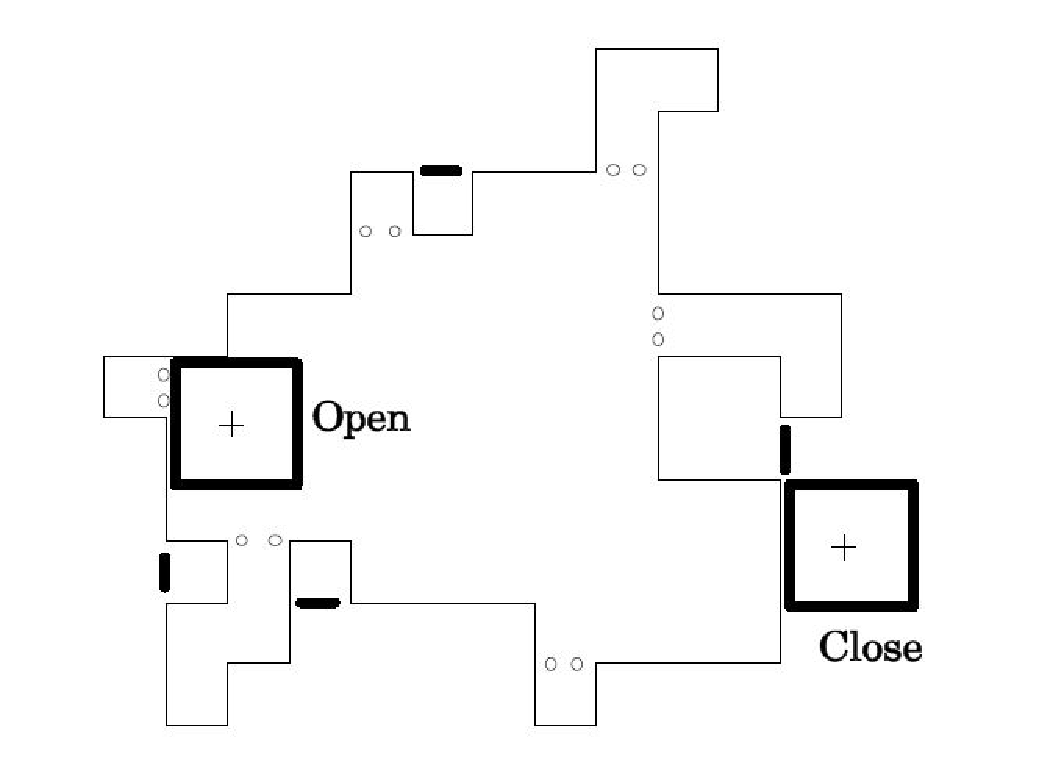
\includegraphics[keepaspectratio,width=0.8\textwidth]{images/4_ZweiteErfahrung/Morphological/oeffnungundschliessung.pdf}
 \caption{Öffnung und Schließung}
 \label{fig:oeffnungundschliessung}
\end{figure} 

\textbf{Schließung}

Genau wie die Öffnung Operation ist die Schließung Operation auch eine Kombination aus Erosion und Dilatation. Der Unterschied dazwischen legt in der Reihenfolge der Operationen, d.h. zuerst wird eine Dilatation Operation, danach eine Erosion Operation mit dem gleichen Strukturelement ausgeführt. Die Schließung eines Bildes A durch das Strukturelement B ist definiert als

\begin{equation}
•A \bullet B =( A \oplus B )\ominus B  
\end{equation}

Die Grenze des geschlossenen Objekts sind die Punkte, wo das Strukturelement B, die äußersten Punkte der Grenze von Objekt erreicht, während B außerhalb dieser Grenze entlangfahren. Kleinere Risse, Lücken und feine Details werden dagegen aufgefüllt und mit den großen Teilen zusammengeschlossen. Abbildung \ref{fig:oeffnungundschliessung} zeigt den Vorgang einer Schließung Operation.


Öffnung und Schließung Operation besitzen folgende Eigenschaften:

\begin{itemize}

\item Öffnung und Schließung sind idempotent.
\item Die Öffnung Operation ist anti-extensiv. 
\item Die Schließung Operation ist extensiv.
\item Öffnung und Schließung sind dual bezüglich der Komplementierung.
\item Ein Bild wird als B-Geöffnet bezeichnet, wenn es bei der gleichen Öffnung Operation unverändert bleibt. 
\item Ein Bild wird als B-Geschlossen bezeichnet, wenn es bei der gleichen Schließung Operation unverändert bleibt. 

\end{itemize}

Das zu detektierendes Bild aus Abbildung \ref{fig:binarisierungbild} nach einer morphologischen Operation wird in Abbildung \ref{fig:Morphological} gezeigt.

\begin{figure}[htb]
 \centering 
  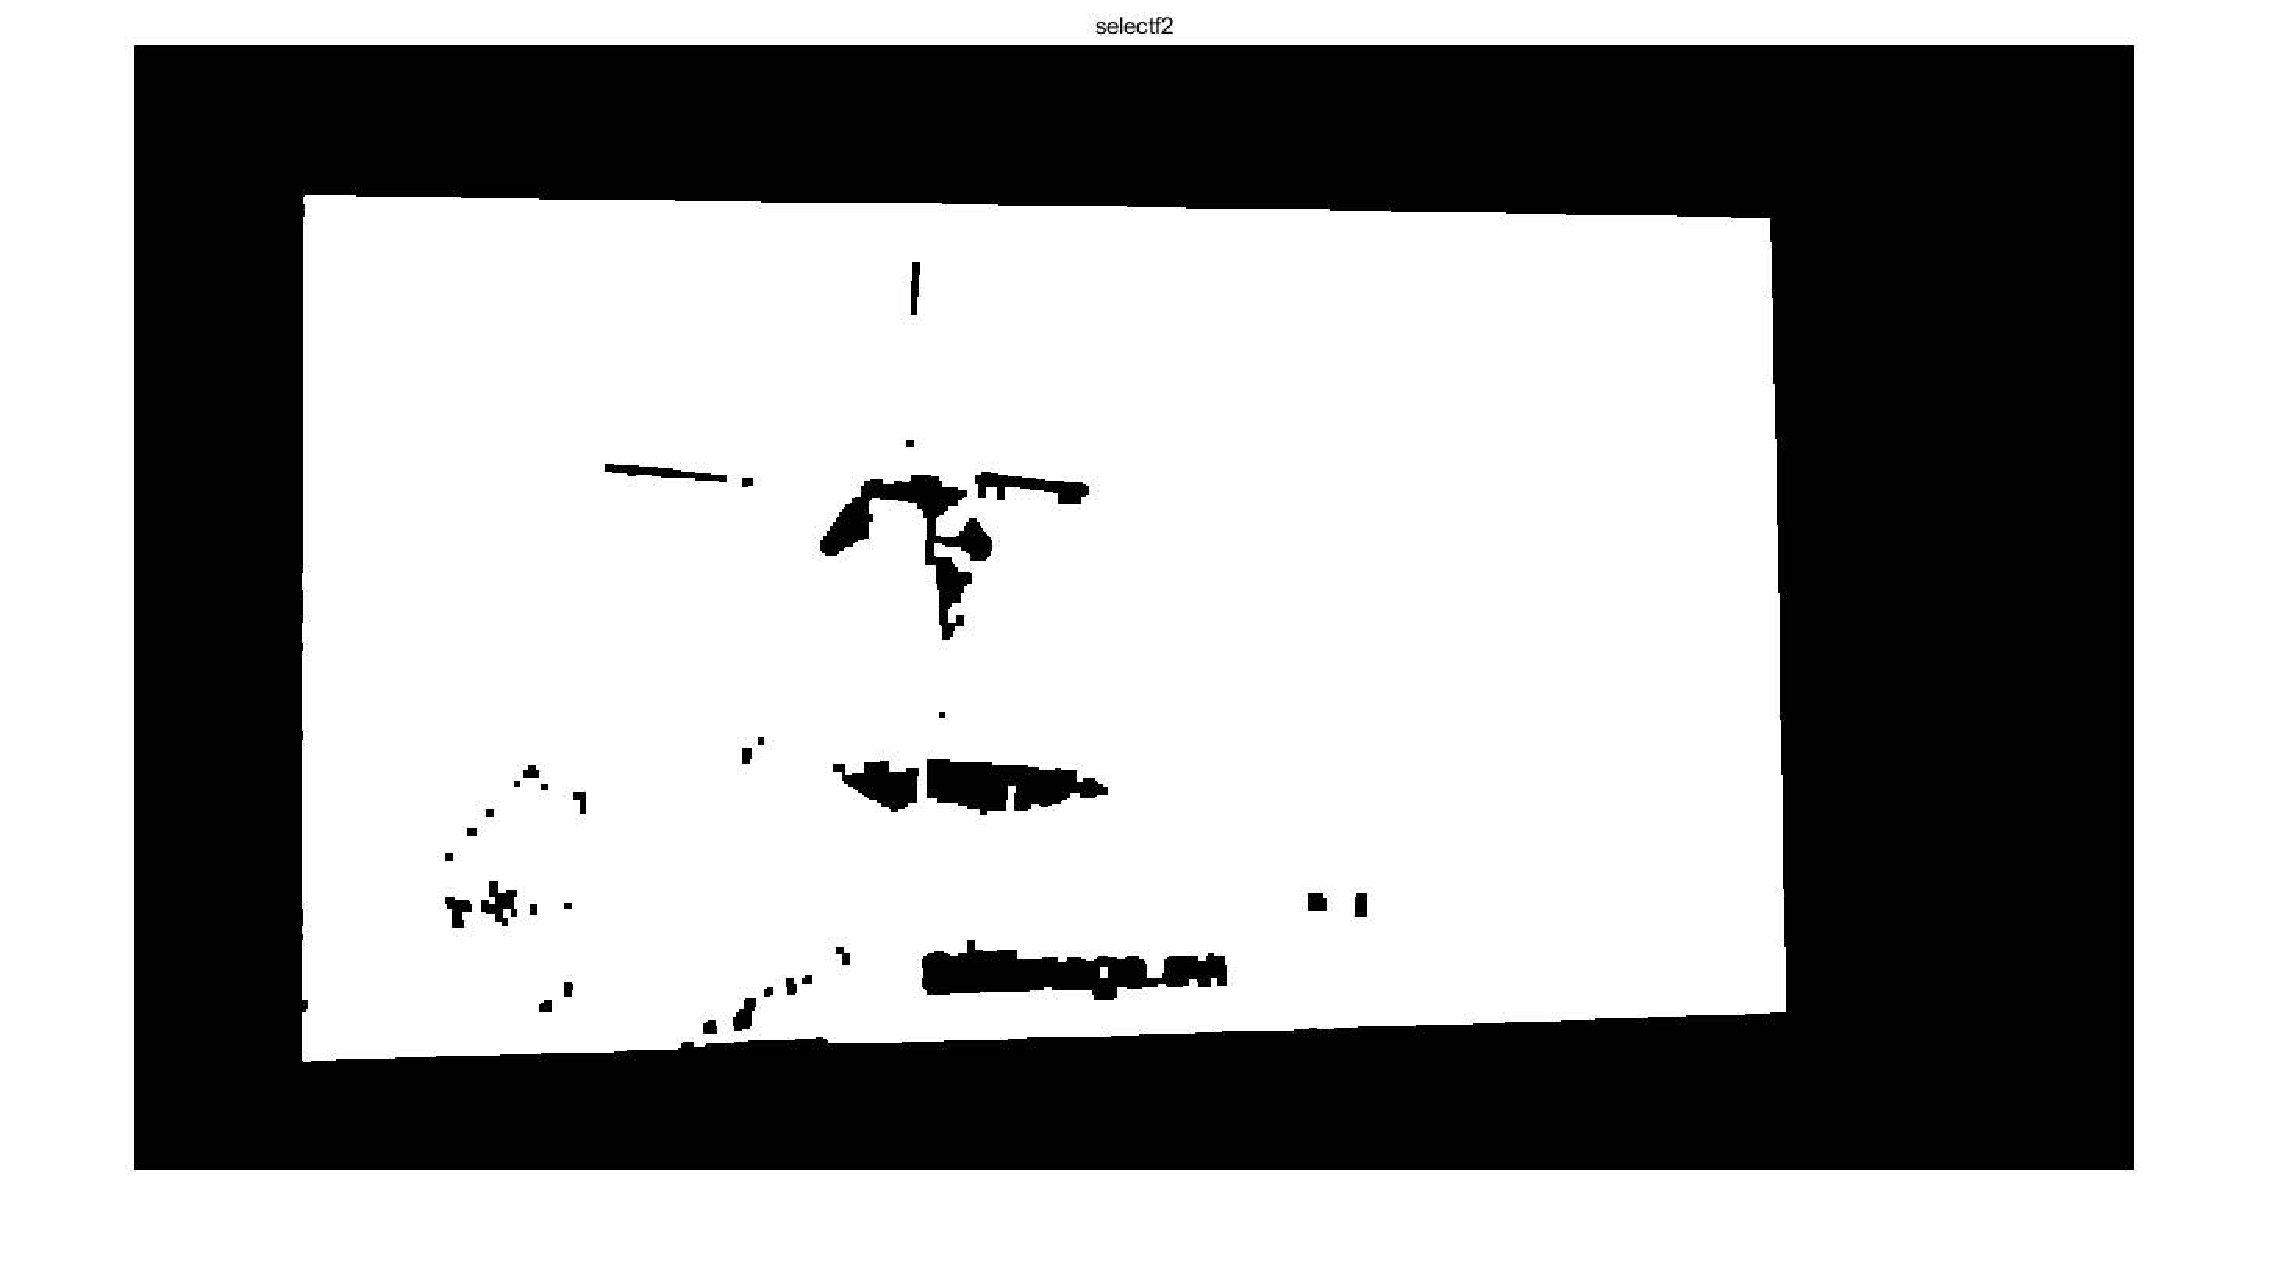
\includegraphics[keepaspectratio,width=1.0\textwidth]{images/4_ZweiteErfahrung/Morphological/morpho.pdf}
 \caption{Bild nach einer morphologischen Operation}
 \label{fig:Bild nach einer morphologischen Operation}
\end{figure} 

\section{Canny detection}

Nach der morphologischen Operation erhalten wir ein Binärbild, welches grob in zwei Teile geteilt werden kann. Ein Modulationsbereich mit dem Pixelwert 1 im mittleren Bereich und einen umgebenden Hintergrundbereich mit dem Pixelwert 0 im äußeren Bereich. Um die nächste Linie Detektion zu implementieren, wird eine Kanten Detektion, weil Kanten oft mit den Grenzen von Objekten in einer Szene verknüpft werden, durchgeführt. In anderen Worten, ist es die Grenze zwischen Modulationsbereich und Hintergrundbereich. \cite{canny}

Es gibt immer einige gut Kantenextraktionsmethode, wie Sobel, Canny, Laplacian, Prewitt, Roberts uvm. In dieser Arbeit wird die leistungsfähigste Kantenerkennungsmethode bzw. der Canny Algorithmus benutzt. Die Canny-Methode unterscheidet sich von den anderen Kantenerkennungsmethoden darin, dass sie zwei verschiedene Schwellenwerte verwendet (um starke und schwache Kanten zu erkennen) und die schwachen Kanten in der Ausgabe nur dann einschließt, wenn sie mit starken Kanten verbunden sind. Diese Methode kann daher im Vergleich zur anderen Methode weniger Wahrscheinlichkeit verfügen, durch Rauschen getäuscht zu werden, und mehr Wahrscheinlichkeit verfügen, echte schwache Kanten zu erkennen.

Das Ziel vom Canny Algorithmus ist es, einen optimalen Kantenextraktionsalgorithmus zu finden. Drei Kriterien für die optimale Kantendetektion werden vorgeschlagen:

\begin{itemize}

\item Gute Erkennung: Der Algorithmus kann so viele tatsächliche Kanten wie möglich im Bild erkennen.
\item Gute Positionierung: Identifizieren der Kanten so nah wie möglich an den tatsächlichen Kanten im Bild.
\item Minimale Antwort: Kanten in einem Bild können nur einmal identifiziert werden, und mögliches Bildrauschen sollte nicht als Kanten erkannt werden.

\end{itemize}

Die Implemetierung des Canny Algorithmus funktioniert so:

\begin{enumerate}
	\item \textbf{Gaußsche Unschärfe.} Das Hauptziel ist, Rauschen zu entfernen. Da Rauschen Hochfrequenzsignalen ähnelt, wird es leicht als eine falsche Kante erkannt. Die Anwendung Gaußscher Unschärfe ist dazu da, um Rauschen zu entfernen und die Erkennung falscher Kanten zu reduzieren. Es sollte beachtet werden, dass ein zu großer Radius einige schwache Kanten nicht erkennen.
	\item \textbf{Berechnen der Größe und Richtung des Gradienten.} Die Kanten des Bildes können in verschiedene Richtungen zeigen. Daher verwendet der klassische Canny Algorithmus vier Gradientenoperatoren, um die Gradienten in horizontaler, vertikaler und diagonaler Richtung zu berechnen. Jedoch werden im allgemeinen diese vier Gradientenoperatoren nicht verwendet, sondern mit Kantenunterschiedsoperatoren (wie Rober, Prewitt, Sobel) die Differenz $ G_x $ und $ G_y $ in horizontaler und vertikaler Richtung berechnet. Die Berechnung der Gradientengröße und Richtung funktioniert wie folgt:	
\begin{equation}
\begin{split}
•  G   & = \sqrt{G_x^{2} + G_y^{2}} \\
\theta & = arctan2(G_y,G_x)
\end{split}
\end{equation}

Der Gradientenwinkel $ \theta $ liegt im Bereich Radianten $ -\pi $ bis $ \pi $, anschließend approximiert dieser in vier Richtungen, die horizontale, vertikale und zwei diagonale Richtungen $(0^{\circ}, 45^{\circ}, 90^{\circ}, 135^{\circ}) $ repräsentieren. Dieser kann durch $  \pm i \pi / 8\ (i =1, 3, 5, 7) $ geteilt werden, sodass der in jeweils einem Bereich fallende Gradientenwinkel einen spezifischen Wert ergibt, der eine von vier Richtungen repräsentiert. Es folgt ein Beispiel einer Sobel Operator.

\begin{equation}
G_x = \begin{bmatrix}
-1 &0 &+1 \\
-2 &0 &+2 \\
-1 &0 &+1
\end{bmatrix} * A \quad and \quad G_y = \begin{bmatrix}
+1 &+2 &+1 \\
0 &0 &0 \\
-1 &-2 &-1
\end{bmatrix} * A
\end{equation}
	
	\item \textbf{Nicht-maximale Unterdrückung.} Nicht-maximale Unterdrückung ist eine Kantenverfeinerungsmethode. Die Gradientenkanten, die normalerweise abgeleitet werden, sind nicht einen, sondern mehrere Pixel breit, während Kriterium 3 erfordert, dass die Kante nur eine genaue Punktbreite hat. Nicht-maximale Unterdrückung kann dazu beitragen, den lokalen maximalen Gradienten beizubehalten, während alle anderen Gradientenwerte unterdrückt werden. Dies bedeutet, dass nur die schärfste Position in der Gradientenänderung beibehalten wird. Der Algorithmus funktioniert wie folgt:
	\begin{itemize}
	\item Vergleichen der Gradientenstärke des aktuellen Punkts mit der Gradientenstärke der positiven und negativen Gradientenrichtungspunkte.
	\item Wenn die Gradientenstärke des aktuellen Punktes im Vergleich zur Gradientenstärke anderer Punkte in der gleichen Richtung am größten ist, wird der Wert auf 1 beibehalten. Ansonsten wird dieser auf 0 gesetzt. Zum Beispiel, wenn die Gradientenrichtung des aktuellen Punktes in die Richtung von $90^{\circ}$ direkt darüber zeigt, muss es mit den Pixeln in der vertikalen Richtung direkt darüber und darunter verglichen werden.
	\end{itemize}
	
	Es ist erwähnenswert, dass die positiven und negativen Richtungen keine unterschiedlichen Bedeutungen haben. Zum Beispiel ist die südöstliche Richtung sowie die nordwestliche Richtung als eine Richtung der Diagonalen zu betrachtet. Vorher approximieren die Gradientenrichtung horizontal, vertikal und zwei Diagonalen in vier Richtungen, so dass jedes Pixel in einer dieser vier Richtungen entsprechend mit seiner eigenen Gradientenrichtung verglichen wird, um zu bestimmen ob es beibehalten wird. 
	
	
	\item \textbf{Doppelte Schwelle.} Ein allgemeiner Kantenerkennungsalgorithmus welcher einen Schwellenwert verwendet, um kleine Gradientenwerte zu entfernen die durch Rauschen oder Farbänderungen verursacht werden, während große Gradientenwerte beibehalten werden.
Der Canny Algorithmus wendet einen doppelten Schwellenwert, d.h. einen hohen und einen niedrigen Schwellenwert an, um Kantenpixel zu unterscheiden. Wenn der Kantenpixelpunktgradientwert größer als der hohe Schwellenwert ist, wird er als ein starker Kantenpunkt betrachtet. Wenn der Kantengradientenwert kleiner als der hohe Schwellenwert und größer als der niedrige Schwellenwert ist, wird er als ein schwacher Kantenpunkt markiert. Punkte, die unterhalb der niedrigen Schwelle liegen werden unterdrückt.

	\item \textbf{Hysterese Grenzenverfolgung.} Bisher könnten die starken Kantenpunkte als echte Kante angesehen werden. Dagegen könnten schwache Kantenpunkte echte Kanten sein, jedoch könnten diese ebenfalls eine Ursache von Rauschen oder Farbänderungen sein. Um genaue Ergebnisse zu erhalten, sollten Kantenpunkte zweiter Art entfernt werden. Im Allgemein werden schwache Kantenpunkte und starke Kantenpunkte die durch reale Kanten verursacht werden, als verbunden betrachtet, während schwache durch Rauschen verursachten Kantenpunkte, keine Verbindung besitzen sind. Der sogenannte Hysterese Grenzenverfolgung Algorithmus untersucht die angrenzenden Pixel eines schwachen Kantenpunktes, solange ein starker Randpunkt vorhanden ist, wird dieser schwache Randpunkt als echter Kantenpunkt betrachtet und wird dessen Wert als 1 geblieben.
	
Zur Implementierung dieses Schritts werden alle verbundenen schwachen Kanten untersucht. Wenn ein Punkt einer verbundenen schwachen Kante mit einem starken Kantenpunkt verbunden ist, wird die schwache Kante beibehalten, ansonsten wird diese schwache Kante unterdrücken. Bei der Suche kann der Algorithmus $ ``Breite zuerst" $ oder $ ``Tiefe zuerst" $ verwendet werden. Nach der gesamten Suche des Bildes, werden die Nicht-Kantenpunkte entfernt, d.h. der Wert dieser auf 0 gesetzt wird.
	
\end{enumerate}

Abbildung \ref{fig:Binärbild nach der Canny detektion} zeigt ein Ergebnis mit der Canny Kantenextraktion.

\begin{figure}[H]
 \centering 
  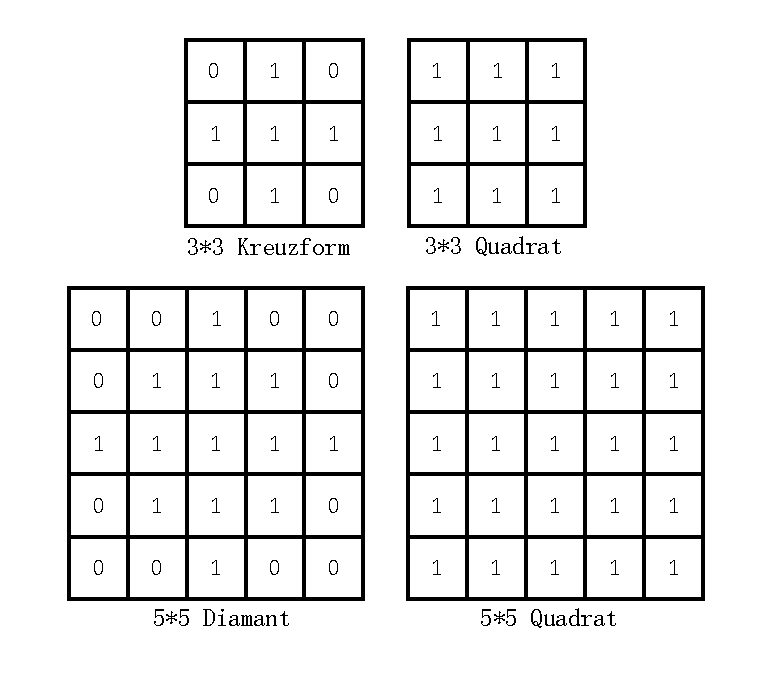
\includegraphics[keepaspectratio,width=1.0\textwidth]{images/4_ZweiteErfahrung/Canny/canny.pdf}
 \caption{Binärbild nach der Canny detektion}
 \label{fig:Binärbild nach der Canny detektion}
\end{figure} 

\section{Cross Dilatation}

Es könnte herausfinden, dass viele Linien aufgrund der Kamera-Verzerrung nicht perfekt gerade sind, wie Abbildung zeigt. Dies kann die Erkennung des Rechtecks in praktischen Anwendungen beeinträchtigen. Um dieses Problem zu lösen und die robuste Leistung der Methode zu erhöhen, Cross Dilatation wird eingeführt, welche jedes Pixel $ (x,y) $ zu einem Kreuzmuster zu erweitern. Alle Pixel, einschließlich die ausdehnte Pixeln, werden zu die nächste Operation behandelt. 

Es ist angenommen, dass die Sphäre des Einflusses jedes Pixels mit einer Region dargestellt wird, die um das Pixel herum zentriert ist und sondern nicht das Pixel selbst. Dann wenn jede Pixel auf eine Linien kann die Region erreichen, die durch das nächste Pixel der Linien beeinflusst wird, dann könnte die gesamte Linie extrahiert werden. Um die Sphäre des Einflusses zu bezeichnen, wird jedes Pixel $ (x,y) $ zu einem Kreuzmuster erweitert, indem ein benachbartes Pixel in der vier Richtung des Pixels 1 setzen, wie in Abbildung 4 gezeigt.

\section{Hough Transformation}

Hier werden die Grenzen des modulierten Rechtecks als Linien betrachtet. Um das Problem für eine Rechteck Detektion lösbar zu machen, müssen zunächst Linie extrahiert werden. Um dies zu tun, müssen die Kanten die auf einer Linie im Bild liegen erkannt werden. Die Hough Transformation ist eine beliebte Methode zum Extrahieren von Linien aus einem Bild. Diese ist in der Lage die benötigten Informationen zu liefern, indem die Spitzen an den Punkten der geraden Linien denen des binären Bildes entsprechen. Der Aufwand einer Hough Transformation hängt von der Größe des Bildes und der Anzahl der analysierten Winkel ab. Da die Winkelauflösung für die weitere Verarbeitung wichtig ist, ist eine maximale Kameraneigung vorgeschrieben, welcher in dieser Arbeit $ \pm 10^{\circ} $ beträgt.

Um die Funktionsweise des HT Algorithmus zu beschreiben, müssen einige Definition eingefügt werden. In der Hough Transformation, kann jede Linie in der $ xy $ Ebene parametrisch beschreiben werden als:
\begin{equation}
•  \rho = x \cos \theta + y \sin \theta
 \label{gl:Anglekoordinate}
\end{equation} 

Hier bedeutet $ \rho $ die Entfernung vom Ursprung der Koordinate zur Linie, $ \theta $ der Winkel zwischen $ \rho $ und der positiven Richtung der x-Achse, $ (x,y) $ sind die Punkte auf der geraden Linie, wie Abbildung \ref{fig:Hough} zeigt.

\begin{figure}[H]
 \centering 
  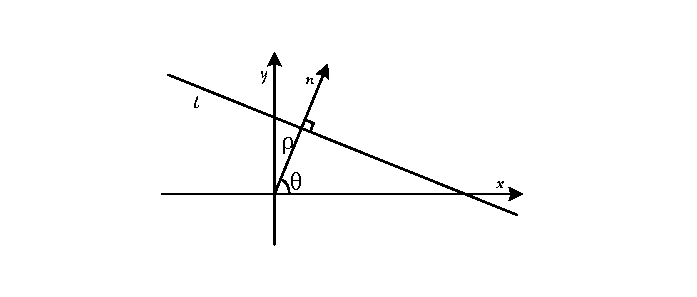
\includegraphics[keepaspectratio,width=1.0\textwidth]{images/4_ZweiteErfahrung/Hough/Hough.pdf}
 \caption{$ \rho,\theta $ Parameterraum}
 \label{fig:Hough}
\end{figure}

Gleichung \ref{gl:Anglekoordinate} gilt für jedes Pixel auf dem Bild, d.h. für jeden Punkt auf dem Bild kann eine entsprechende trigonometrische Kurve nach der Hough-Transformation im Parameterraum ($ \theta $, $ \rho $) gefunden werden. Es werden zufällig zwei Punkte auf dem Bild ausgesucht, die zwei  trigonometrischen Kurven entsprechen welche unvermeidlich einen Schnittpunkt ($ \theta_0 $, $ \rho_0 $) erzeugen werden. Dieser Schnittpunkt wird dann in die Gleichung der Linie eingefügt, um eine gerade Linie zu bestimmen (und zwar die durch die zwei Punkte auf dem Bild festgelegte Linie). 

Das heißt, die entsprechenden trigonometrischen Kurven, die von Punkten auf derselben Linie auf dem Bild erzeugt werden, schneiden sich an einem Punkt ($ \theta_0 $, $ \rho_0 $) im Parameterraum. Je mehr Punkte auf der Linie sind, desto mehr Kurven schneiden sich an diesem Punkt. Wie der Algorithmus einer Hough Transformation wie folgendermaßen darstellt:

\begin{enumerate}
\item Erstellung eines Parameterraums mit einer geeigneten Quantisierungsstufe für Entfernung $ \rho $ und Winkel $ \theta $.
\item Erstellung eines Akkumulator Array A($ \rho $,$ \theta $) für alle ($ \rho $,$ \theta $).
\begin{equation}
A(\rho,\theta) = 0
\end{equation}
\item Für jeden Nicht-Hintergrundpunkt $ (x,y) $ wird im Bild $ \rho $ mit jedem $ \theta $ berechnet, ob diese Gleichung erfüllt wird: $ \rho = x \cos \theta + y \sin \theta $. Wird das Akkumulator-Array um 1 erhöht: 
\begin{equation}
 A(\rho,\theta) = A(\rho,\theta) + 1 
\end{equation}
\item Suche des Spitzenwerts im Array A, welche die Linie im Parameterraum angibt.
\end{enumerate}

Eine Beispiel Implementierung der Hough Transformation ist in Abbildung \ref{fig:Houghdetektion} zu sehen.

\begin{figure}[H]
 \centering 
  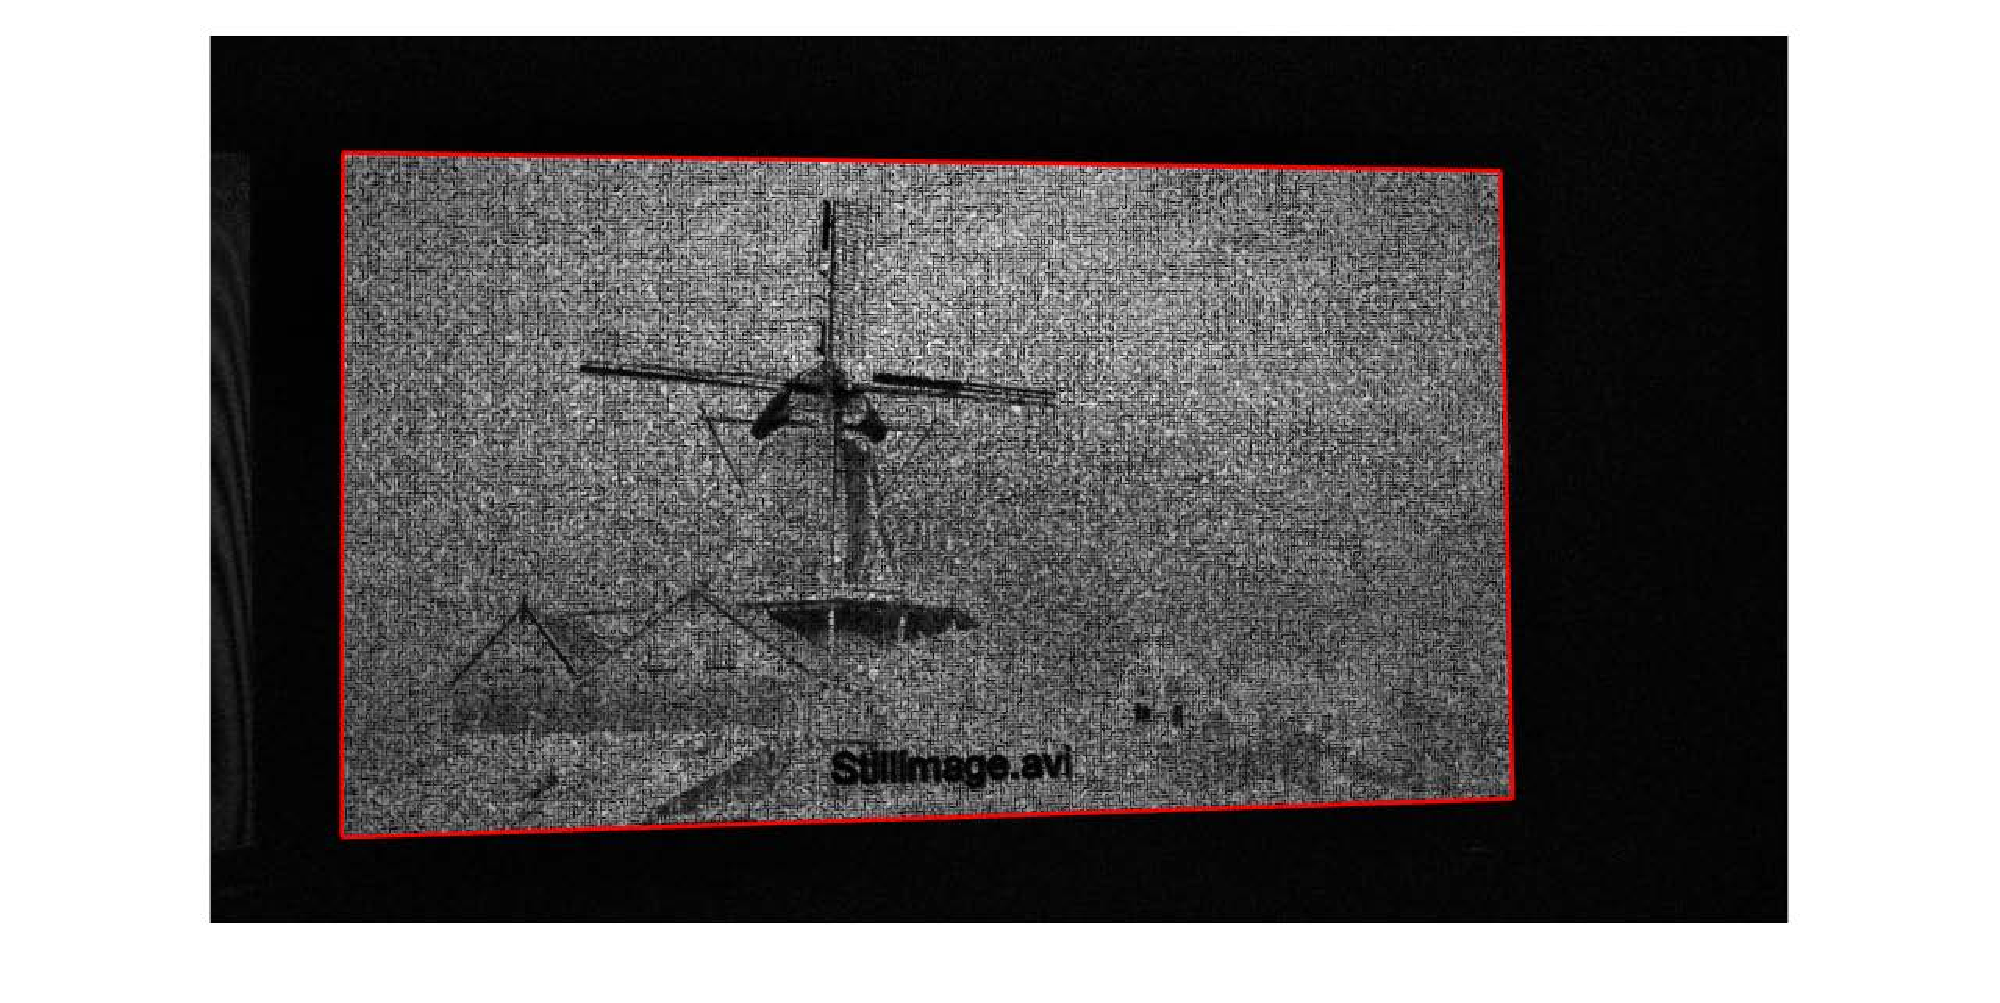
\includegraphics[keepaspectratio,width=1.0\textwidth]{images/4_ZweiteErfahrung/Hough/Houghdetektion.pdf}
 \caption{Houghdetektion}
 \label{fig:Houghdetektion}
\end{figure}

\section{Radon Transformation}
In diesem Abschnitt wird eine erweiterte Form von Hough Transformation bzw. Radon Transformation vorgestellt. Die Hough Transformation transformiert eine gegebene Kurve im Bildraum als ein Punkt im Parameterraum entsprechend dem Parameterausdruck der Kurve ,dann durch Suchen nach Peaks in dem Parameterraum diesen Kurve in dem Bildraum bestimmen. Radon Transformation projiziert den Bildraum in den $ \rho \theta $-Raum in Form eines Linienintegrals (entspricht dem Parameterraum der Linie). Es kann verstanden werden, dass die Hough Transformation eine diskrete Form der Radon Transformation ist. Aufgrund der soliden mathematischen Basis ist die Radon Transformation  im Gegensatz dazu raffinierter und genauer.

Die Idee der Radon-Transformation besteht darin, die ursprüngliche Funktion räumlich zu transformieren, das heißt, die ursprünglichen in der XY-Ebene Punkte werden auf die AB-Ebene abgebildet. Dann sind alle Punkte einer geraden Linie in der XY-Ebene an einer demselben Punkt der AB-Ebene. Zeichnen die akkumulierte Dicke der Punkte auf der AB-Ebene auf, und können die Existenz der Linien auf der XY-Ebene kennen.

Wie bei der Hough-Transformation werden die Parameter $ \rho $ und $ \theta $ zuerst verwendet, um die gerade Linie auf der xy-Ebene darzustellen. Diese Parametrisierte Linie wird in Abbildung \ref{fig:Parametrisierte Linie} gezeigt und die Formel läuft als:
\begin{equation}
•  L(\rho,\theta)=\lbrace(x,y):x\cos{\theta} + y\sin{\theta} = \rho\rbrace
\end{equation} 

Angenommen, es gibt eine Funktion f (x, y), wie in Abbildung \ref{fig:Integral der Funktion f (x, y)} gezeigt, dann ist das Integral der Funktion über die gerade Linie L:
\begin{equation}
•  \int_{L}= f(x,y)\ ds
\end{equation} 
Wobei $ ds $ das Differential der Linie ist. 

\begin{figure}[H]
\centering 
\begin{minipage}[b]{0.49\textwidth} 
\centering 
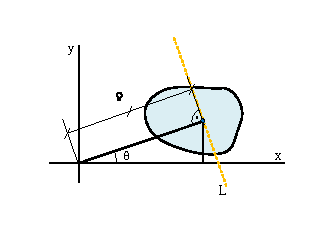
\includegraphics[width=1.0\textwidth]{images/4_ZweiteErfahrung/Radon/1.pdf} 
\caption{Parametrisierte Linie}
\label{fig:Parametrisierte Linie}
\end{minipage}
\begin{minipage}[b]{0.49\textwidth} 
\centering 
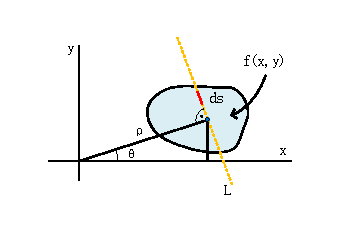
\includegraphics[width=1.0\textwidth]{images/4_ZweiteErfahrung/Radon/2.pdf}
\caption{Integral der Funktion $ f(x,y) $}
\label{fig:Integral der Funktion f (x, y)}
\end{minipage}
\end{figure}

Die obigen Integrale für x, y sind leicht zu lösen. Eine der Lösungstechniken ist die Verwendung der Delta-Funktion. Das obige Integral kann geschrieben werden als:
\begin{equation}
•  \int_{-\infty}^{\infty} \int_{-\infty}^{\infty} f(x,y)\delta (x\cos{\theta} + y\sin{\theta}-\rho)\ dxdy
\end{equation} 
Deswegen wenn einen Satz von $ (\rho,\theta) $ bestimmen, können einen Integral Wert entlang $ L(\rho,\theta) $ erhalten. Somit wird die Radon-Transformation zum Linienintegral der Funktion $ f(x,y) $ umgewandelt, wie in Abbildung \ref{fig:Radon Transformation als Linienintegral} gezeigt. Die Höhe $ g $ repräsentiert das Linienintegral von $ f(x,y) $ auf der Linie L.

\begin{figure}[H]
\centering 
\begin{minipage}[b]{0.49\textwidth} 
\centering 
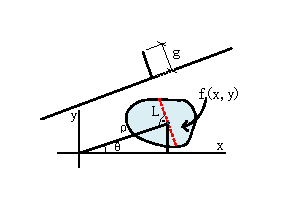
\includegraphics[width=1.0\textwidth]{images/4_ZweiteErfahrung/Radon/3.pdf} 
\caption{Radon Transformation als Linienintegral}
\label{fig:Radon Transformation als Linienintegral}
\end{minipage}
\begin{minipage}[b]{0.49\textwidth} 
\centering 
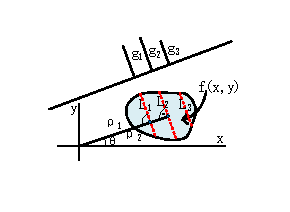
\includegraphics[width=1.0\textwidth]{images/4_ZweiteErfahrung/Radon/4.pdf}
\caption{Parallele Linienintegral mit gleichen $ \theta $}
\label{fig:Parallele Linienintegral}
\end{minipage}
\end{figure}

Wenn viele Linien parallel zu L sind, haben sie das gleiche $ \ theta $, die radialen Koordinaten $ \ rho $ sind verschieden. Für jede solche parallele Linie machen ein Linienintegral von f (x, y), werden viele Projektionslinien erzeugt, wie in Abbildung \ref{fig:Parallele Linienintegral} gezeigt. Das heißt, die Radon-Transformation eines Bildes in einem bestimmten Winkel erzeugt N Linienintegralwerte (Radon-Transformation), und jeder Zeilenintegralwert entspricht einer Radialkoordinate. Die Radon-Transformationswerte bei verschiedenen Winkeln werden kombiniert, um ein Radon-Diagramm zu bilden.

